\section*{Случайные блуждания}
\addcontentsline{toc}{section}{Случайные блуждания}
\subsection*{Одномерный дискретный случай}
\addcontentsline{toc}{subsection}{Одномерный дискретный случай}

\textbf{Задание:}\\
Реализовать модель процесса случайного блуждания. Рассчитать среднеквадратическое отклонение, размах в определённом интервале и математическое ожидание. Построить гистограмму по получаемым координатам. Визуализировать процесс перемещения точки.\\

\textbf{Решение:}\\
В качестве вероятности перемещения вверх или вниз была задана вероятность 0.5. Начальная точка была взята 0, количество наблюдений -- 1000. В соответствии с процессом случайного блуждания был промоделирован процесс. (Рисунок \ref{fig:random_walk1})
\begin{figure}[h]
	\centering 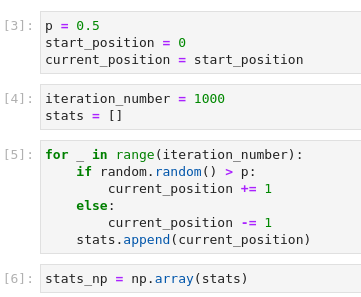
\includegraphics[scale=0.5]{random_walk1}
	\caption{Моделирования процесса случайного блуждания}
	\label{fig:random_walk1}
\end{figure}

Были рассчитаны основные показатели модели. (Рисунок \ref{fig:random_walk2},  \ref{fig:random_walk3})
\begin{figure}[h]
	\centering 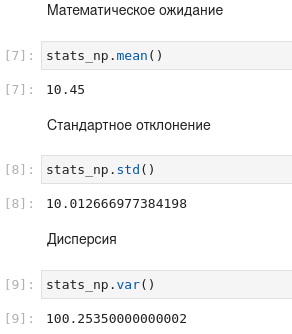
\includegraphics[scale=0.4]{random_walk2}
	\caption{Основные показатели модели}
	\label{fig:random_walk2}
\end{figure}

\newpage

\begin{figure}[h]
	\centering 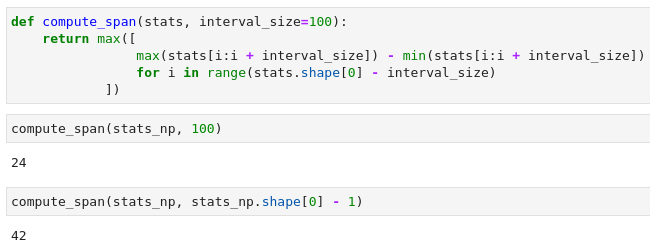
\includegraphics[scale=0.6]{random_walk3}
	\caption{Вычисление размаха}
	\label{fig:random_walk3}
\end{figure}

Также был визуализирован процесс перемещения точки с течением времени. (Рисунок \ref{fig:random_walk4})
\begin{figure}[h]
	\centering 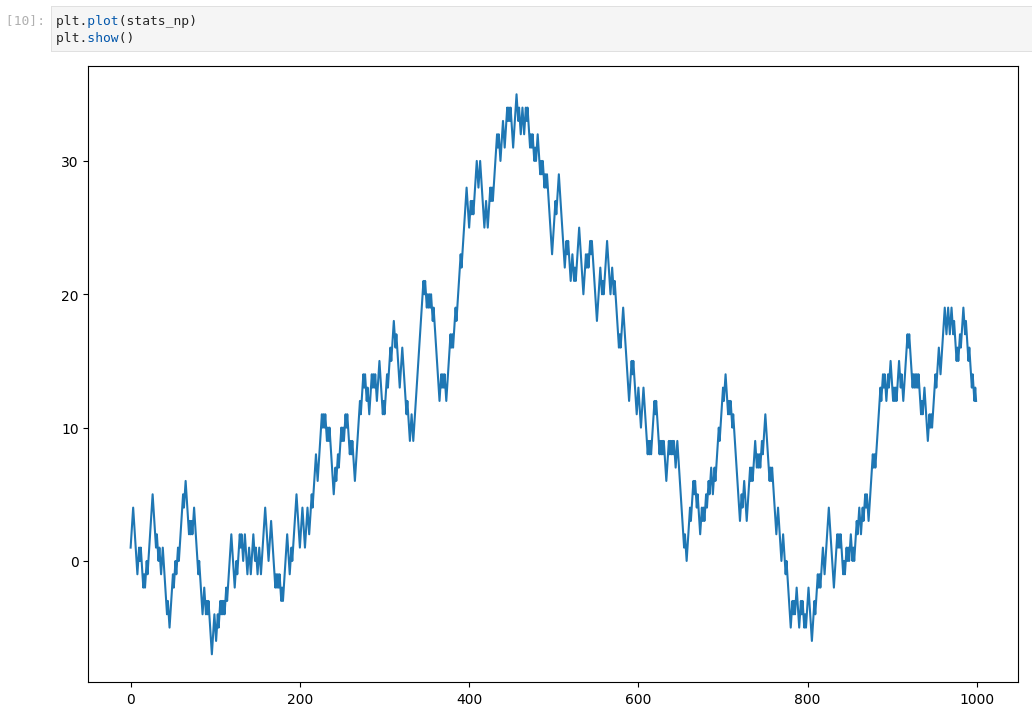
\includegraphics[scale=0.4]{random_walk4}
	\caption{Визуализация процесса перемещения точки с течением времени}
	\label{fig:random_walk4}
\end{figure}

\newpage

Ещё была построена гистограмма, на которой показана частота встречаемости значений. (Рисунок \ref{fig:random_walk5})

\begin{figure}[h]
	\centering 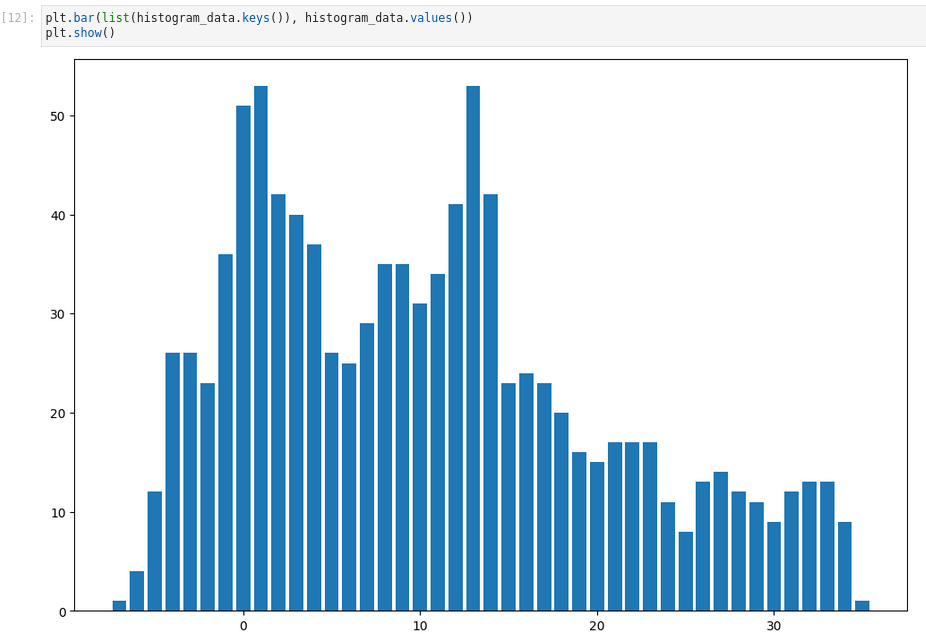
\includegraphics[scale=0.4]{random_walk5}
	\caption{Гистограмма по частоте встречаемости значений}
	\label{fig:random_walk5}
\end{figure}

Таким образом, был рассмотрен процесс случайных блужданий для одномерного дискретного случая.